\chapter{A data mining framework for automatic event detection and summarisation}
\ifpdf
    \graphicspath{{Chapter2/Chapter2Figs/PNG/}{Chapter2/Chapter2Figs/PDF/}{Chapter2/Chapter2Figs/}}
\else
    \graphicspath{{Chapter2/Chapter2Figs/EPS/}{Chapter2/Chapter2Figs/}}
\fi

In this chapter we will define a theoretical framework for construction of a 
data mining system which can extract events from Twitter data. The system comprises of a number
of individual components which when combined together construct a complete framework for 
event extraction. These components are explained in detail in the sections below and in 
Chapter \ref{chap:Application} we discuss the concrete implementation of this framework as 
well as the development of a proof-of-concept application using this framework.\\
The first section of this chapter introduces the motivating work for the implementation of the system
and we take a closer look at the concepts and key ideas that are necessary to understand the process we employ.

\section{Methodology overview}\label{MethodologyOverview}
The main idea behind our methodology for event detction is that similar events will be described by tweets having similar
content. Therefore, the main task in our methodology is to cluster the tweets in different groups. Having done that
we can then further investigate these clusters and identify which ones are events and also extract useful information from them.
This procedure is described in detail in the rest of this chapter and Figure 3.1 depicts an overview of the system. 
Initially, historical tweets from a service provider (Twitter API or another provider) should be retrieved and stored in an 
appropriate format in the database. Subsequently, the system receives a stream of tweets from the database and process and 
transforms them in a format that is appropriate for clustering. The next step in the pipeline is the actual clustering of the tweets 
in order to detect groups of tweets discussing the same topic. Then, the extracted clusters are processed in order to identify the events 
and generate their summaries. Finally, a visual representation of the results should be generated in order to aid understanding of the events.\\

In our discussion in this chapter we will leave out the data retrieval aspect since it is dependent on the actual implementation and it 
will be described in detail in Chapter \ref{chap:Application}. For now we'll assume that we have a source of tweets,such as the Twitter API which provides 
us a collection of historical tweets. 

\begin{figure}[!htbp]
  \begin{center}
    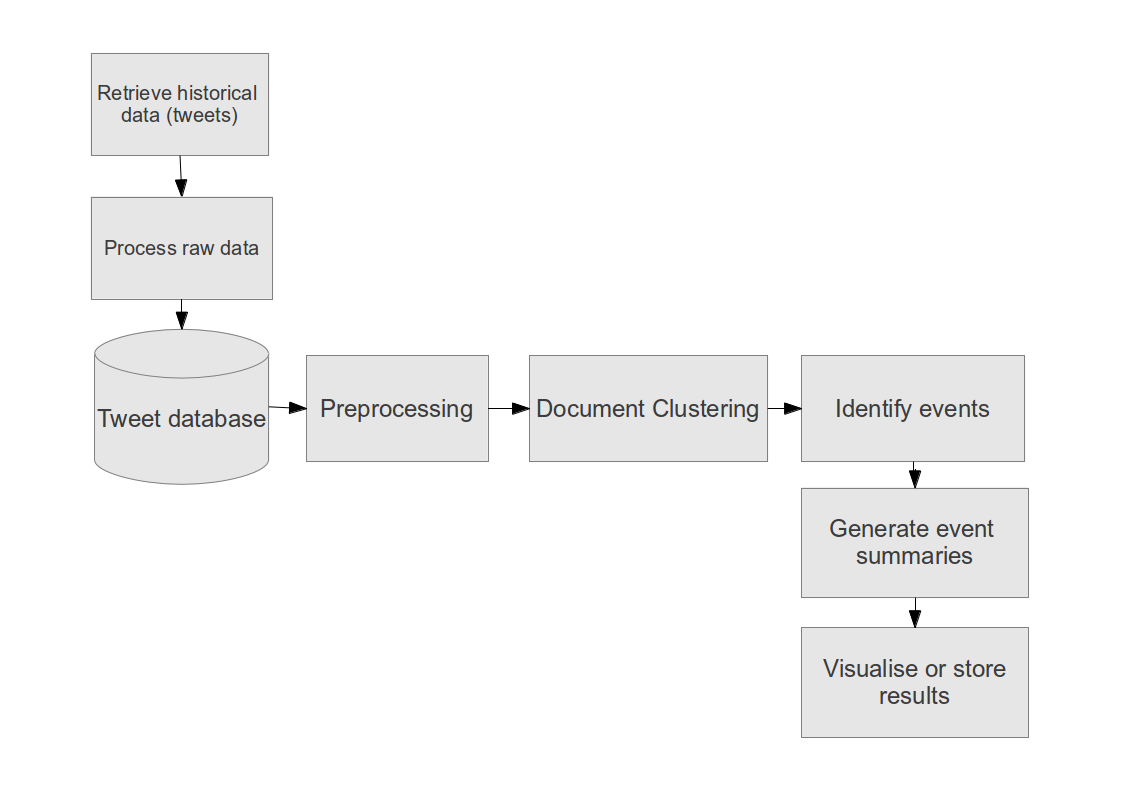
\includegraphics[height=3in, width=6in]{system-overview}
    \caption{System overview - The event extraction system comprises of several independent components.}
    \label{SystemOverview}
  \end{center}
\end{figure}

\section{Raw data processing}\label{RawDataProcessing}
Mining and analysing text corpora are two well studied problems but in our case we face a slightly
different problem. Social media content and especially tweets are very short (140 characters)
and usually contain slang phrases, abbreviations and irrelevant information. Therefore, is of
foremost importance to ensure that clever data preprocessing takes place in order to help us in
the subsequent tasks. 

\begin{figure}[!htbp]
  \begin{center}
    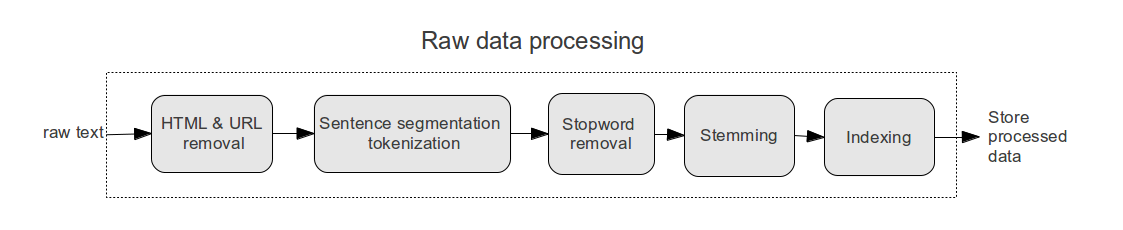
\includegraphics[height=1.5in, width=6in]{raw-data-processing}
    \caption{The raw data processing module - All the steps neccessary to convert raw documents to a format suitable for storage in a database.}
    \label{RawDataProcessingOverview}
  \end{center}
\end{figure} 

\subsection{Natural language processing}

Natural language processing (NLP) is a field of computer science and linguistics which is concerned with the extraction of information from a human language 
input. NLP is used extensively throughout this project since we deal with human generated content and we use several of its applications. NLP in the context 
of raw data processing is used to clean and normalise our initial input which is a tweet containing raw text.\\ 
Since tweets usually contain URLs and HTML code one of the first priorities is to remove these elements. Then, the following NLP algorithms
can be used on our data:

\begin{itemize}
 \item Sentence segmentation and tokenization: Raw text is split into sentences and then each sentence is further subdivided into words using a tokenizer. 
 \item Stopword removal: Some of the words occuring in the documents are common English words such as 'the', 'and' and 'a'. These words convey almost no information 
 but most importantly, they can reduce the clustering accuracy. Two documents can be erroneusly considered related if they contain common English words like the ones
  we have already mentioned. Therefore, it is important to remove these stopwords. Usually, a dictionary of the common English stopwords is used to filter them out.   
 \item Stemming: This is a mechanism for reducing English words to their stem form. For example, the stem form of the words `connections' and `connected' is `connect'. This    mechanism is particularly useful in the field of information retrieval and indexing. M.F Porter designed the most widely used stemming algorithm in 1980 [Insert ref here]. This algorithm works by applying a set of different rules, which after a number of iteration yield the final resut which is the stem of the word. Porter
has developed 62 rules which may or may not apply to a given word.
\end{itemize}\vspace{15pt}

In section \ref{chap:SummaryGen} we explore more applications of NLP and how we can use them to extract automatic summaries, named entities or sentiment from documents.

\subsection{Inverted index}
An inverted index, also known as an inverted file, is a data structure central to text-based information retrieval. The name is derived from its 
purpose and design which is to map key-value pairs, where a key is a term in a document and the value is the list of documents that contain this term.
For example if we have two documents:\\
\emph{Document1}: The cat is on the tree. \\
\emph{Document2}: The cat sat on the mat. \\
then the inverted index will look like:

\begin{center}
\begin{tabular}{ |l | l| }
  \hline
  \textbf{Key} & \textbf{Value} \\ \hline
  the & \{Document1, Document2\} \\
  cat & \{Document1, Document2\} \\
  is & \{Document1\} \\
  on & \{Document1, Document2\} \\
  tree & \{Document1\} \\
  sat & \{Document2\} \\
  mat & \{Document2\} \\
  \hline
\end{tabular}
\end{center}

The main reason for using an index is to increase the speed and efficiency of searches of the document 
collection. In our system the inverted index is vital component since it allows us to construct
term-documment vectors easily and also filter terms and documents. For example, using our index we
can find the words that appear either too often or less frequently and filter them out. This is used
to reduce the dimensionality of our dataset by removing unneccesary words. Alternatively, we
can remove documents/tweets which contain keywords that appear too often or less frequently.

\section{Clustering}

TODO Avrio: Grapse mia eisagwgi gia to clustering j an theleis grapse ta requirements t clustering..etsi wste na
sindeseis ta algorithms ..taxa "these are the algos that fulfill our reqs"..vale eikonoues gia oulla

Clustering is the process of grouping a set of data objects into multiple clusters where all the
objects in a cluster have high similarity but they are very dissimilar to objects in other clusters.
Dissimilarities and similarities are calculated based on the attribute values of each data object
and they often involve distance measures. Clustering is an unsupervised learning method since
the object labels are not known beforehand.
In our project we are interested in clustering because we would like to cluster tweets which
are similar in terms of both textual content and social content. Additionally, due to the fact
that we have to deal with vast amount of data we are interested in scalability and performance.

\subsection{Vector space representation}

Find a suitable place for this paragraph:
-----------------------------------------
Preprocessing is also required to transform the documents (tweets) in a form that
will allow us to perform clustering on them. Therefore,  we define 'preprocessing' as all tasks which take place before transforming
the documents into the vector space representation. Figure 3.2 show the sub-components of the preprocessing module.

We can represent each document in a dataset by a vector of identifiers. Usually, these identifiers are the distinct words in the document and 
the resulting vector is called term-frequency vector. If we combine all the vectors for the documents in our dataset we will end up with an 
\boldmath $m \times n$  \unboldmath  matrix \boldmath $A$ \unboldmath. Each of the $m$ documents in the document collection are assigned a row 
in the matrix, while each of the $n$ unique terms in each document are assigned a column in the matrix. A non-zero element $a_{ij}$ in \boldmath 
$A$ \unboldmath, indicates not only that term $j$ occurs in document $i$, but also the number of times the term appears in that document. Since the number of terms in a given 
document is typically far less than the number of terms in the entire document collection, A is usually very sparse.\\
For example in Table 3.1 we see that $Document1$ contains three instances of the word team, while football occurs five times. We can also infer that
the words ball and world are missing for the entire document, as indicated by the value of zero at those entries of the matrix.  

The main advantage of transforming the documents in the vector space is that we can define vector-space similarities between documents and therefore
we can apply clustering algorithms on the document collection. In section we provide a more detailed discussion on similarity metrics and the vector space 
representation is used in clustering documents.

\begin{table}[tbp]
\centering
\begin{tabular}{ l  l  l  l  l  l  l }
  \hline
  \textbf{Document} & \textbf{team} & \textbf{ball} & \textbf{football} & \textbf{countries} & \textbf{world} & \textbf{england} \\ \hline
  \emph{Document1} & 3 & 0 & 5 & 1 & 3 & 1 \\
  \emph{Document2} & 2 & 1 & 2 & 0 & 8 & 2\\
  \emph{Document3} & 1 & 5 & 3 & 0 & 1 & 3\\
  \emph{Document4} & 5 & 0 & 1 & 2 & 5 & 4\\
  \hline
\end{tabular}
\caption{Term-frequency vector representation of documents}
\label{termfrequencyTable}
\end{table}

\subsection{Assigning weights to terms with TF-IDF weighting}
Once a document is transformed in its term-frequency vector we can assign weights to each term in the vector. So far the term-frequency vectors treat 
all the terms as equal but this may not be the case. For example, a word that appears more frequently than others in a document could be considered as an 
important word. At the same time words that appear frequently in the corpus, such as 'a', 'the', 'and', are not very useful and their 
importance must be discounted. \\
The most common method to solve this problem is the TF-IDF weight (TF-IDF stands for term frequency-inverse document frequency) which quantifies the importance of a term in a document of a document collection. More specifically, the more a word occurs in a document, and the less it occurs in the rest of the coprus, the higher its TF-IDF weighting 
will be. Mathematically, TF-IDF is expressed as:\\
\begin{eqnarray}
tf-idf_{t,d} = tf_{t, d} \times idf_t
\end{eqnarray}

where $tf_{t, d}$ is the importance of term $t$ in document $d$ and $idf_t$ is the importance of term $t$ relative to the entire corpus. $tf_{t,d}$ is higher when the term occurs many times in the document and $idf_t$ is higher when it occurs rarely in the dataset. Therefore, the TF-IDF weighting for a term is very high if the term occurs frequently in a single document but very rarely in the entire corpus and it is low when the term either occurs rarely in a document or frequently in the entire corpus. TF-IDF is widely used to compare the similarity between documents and a common use case is for search queries where the similarity of a query $q$ with a document $d$ is calculated using TF-IDF, providing
a sorted list of the most relevant documents. 
\\
   
\subsection{Feature selection}
TODO: Discusss feature selection methods used in our system.


\subsection{Kmeans algorithm}

\subsection{DBSACN algorithm}

\subsection{Non-negative matrix factorisation algorithm}

\subsection{Online clustering algorithm}

\section{Automatic text summaries}\label{SummaryGen}

\subsection{Background}

\subsection{Generating automatic document cluster summaries}

\subsection{Detecting sentiment, named entities and locations in documents}

\section{Twitter user classification}

\subsection{Background}

\subsection{Decision trees}

\subsection{Neural networks}

\section{Summary}

Show a simple diagram with a lot of tweets becoming vectors and then those becoming clusters and then some of them events.
This is the outout of the algorithm.

% ------------------------------------------------------------------------

%%% Local Variables: 
%%% mode: latex
%%% TeX-master: "../thesis"
%%% End: 
